% Created 2012-10-17 Wed 11:30
\documentclass[bigger]{beamer}
\usepackage[utf8]{inputenc}
\usepackage[T1]{fontenc}
\usepackage{fixltx2e}
\usepackage{graphicx}
\usepackage{longtable}
\usepackage{float}
\usepackage{wrapfig}
\usepackage{soul}
\usepackage{textcomp}
\usepackage{marvosym}
\usepackage{wasysym}
\usepackage{latexsym}
\usepackage{amssymb}
\usepackage{hyperref}
\tolerance=1000
\titlegraphic{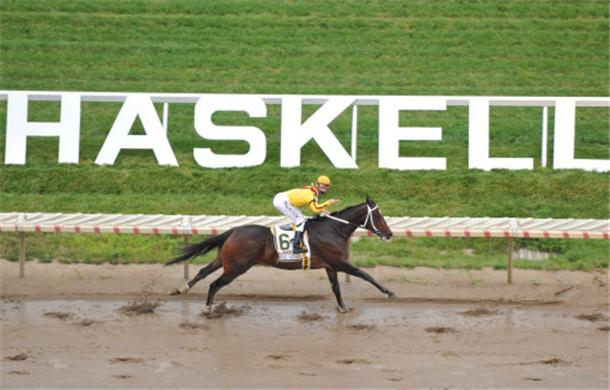
\includegraphics{../pictures/haskell_horse.jpg}}
\setbeamertemplate{navigation symbols}{}
\mode<beamer>{\usetheme{CambridgeUS}}
\institute{GWU}
\providecommand{\alert}[1]{\textbf{#1}}

\title{Pony: Demo 1}
\author{Andrew Hirsch}
\date{2012-10-17 Wed}

\begin{document}

\maketitle


\begin{frame}
\frametitle{Idea}
\label{sec-1}



\begin{itemize}
\item Create a small, extensible calculator language
\item Using techniques that will be used in extensibility of Pony
\end{itemize}
\end{frame}
\begin{frame}
\frametitle{The Language}
\label{sec-2}



\begin{itemize}
\item A simple language: Addition and Subtraction
\item Stack-based language; it's easier to parse
\item + - 3 2 3 = (3 - 2) + 3
\end{itemize}
\pause

\begin{itemize}
\item A simple extension: multiplication
\item * + - 3 2 3 4 = ((3 - 2) + 3) * 4
\end{itemize}
\end{frame}
\begin{frame}
\frametitle{Libraries}
\label{sec-3}



\begin{itemize}
\item Data.Comp
\begin{itemize}
\item Compositional datatypes
\item based off of data types a la carte
\item VERY difficult library
\end{itemize}
\item Text.ParserCombinators.Parsec
\begin{itemize}
\item Parser combinator library
\item Builds parsers from smaller parsers
\item Parsec 2: much simpler internal structure than Parsec 3
\end{itemize}
\end{itemize}
\end{frame}
\begin{frame}
\frametitle{Technical Difficulties}
\label{sec-4}



\begin{itemize}
\item The two libraries do NOT like to play together
\item Compositional datatype-based evaluation is picky about when it will evaluate
\item Composing parsers is unsolved
\begin{itemize}
\item Luckily, it looks like it might be easier than we thought.
\end{itemize}
\end{itemize}
\end{frame}

\end{document}
